\documentclass{standalone}
\usepackage{tikz}
\usetikzlibrary{patterns, positioning}
\usepackage[sfdefault]{ClearSans} %% option 'sfdefault' activates Clear Sans as the default text font
\usepackage[T1]{fontenc}

\begin{document}
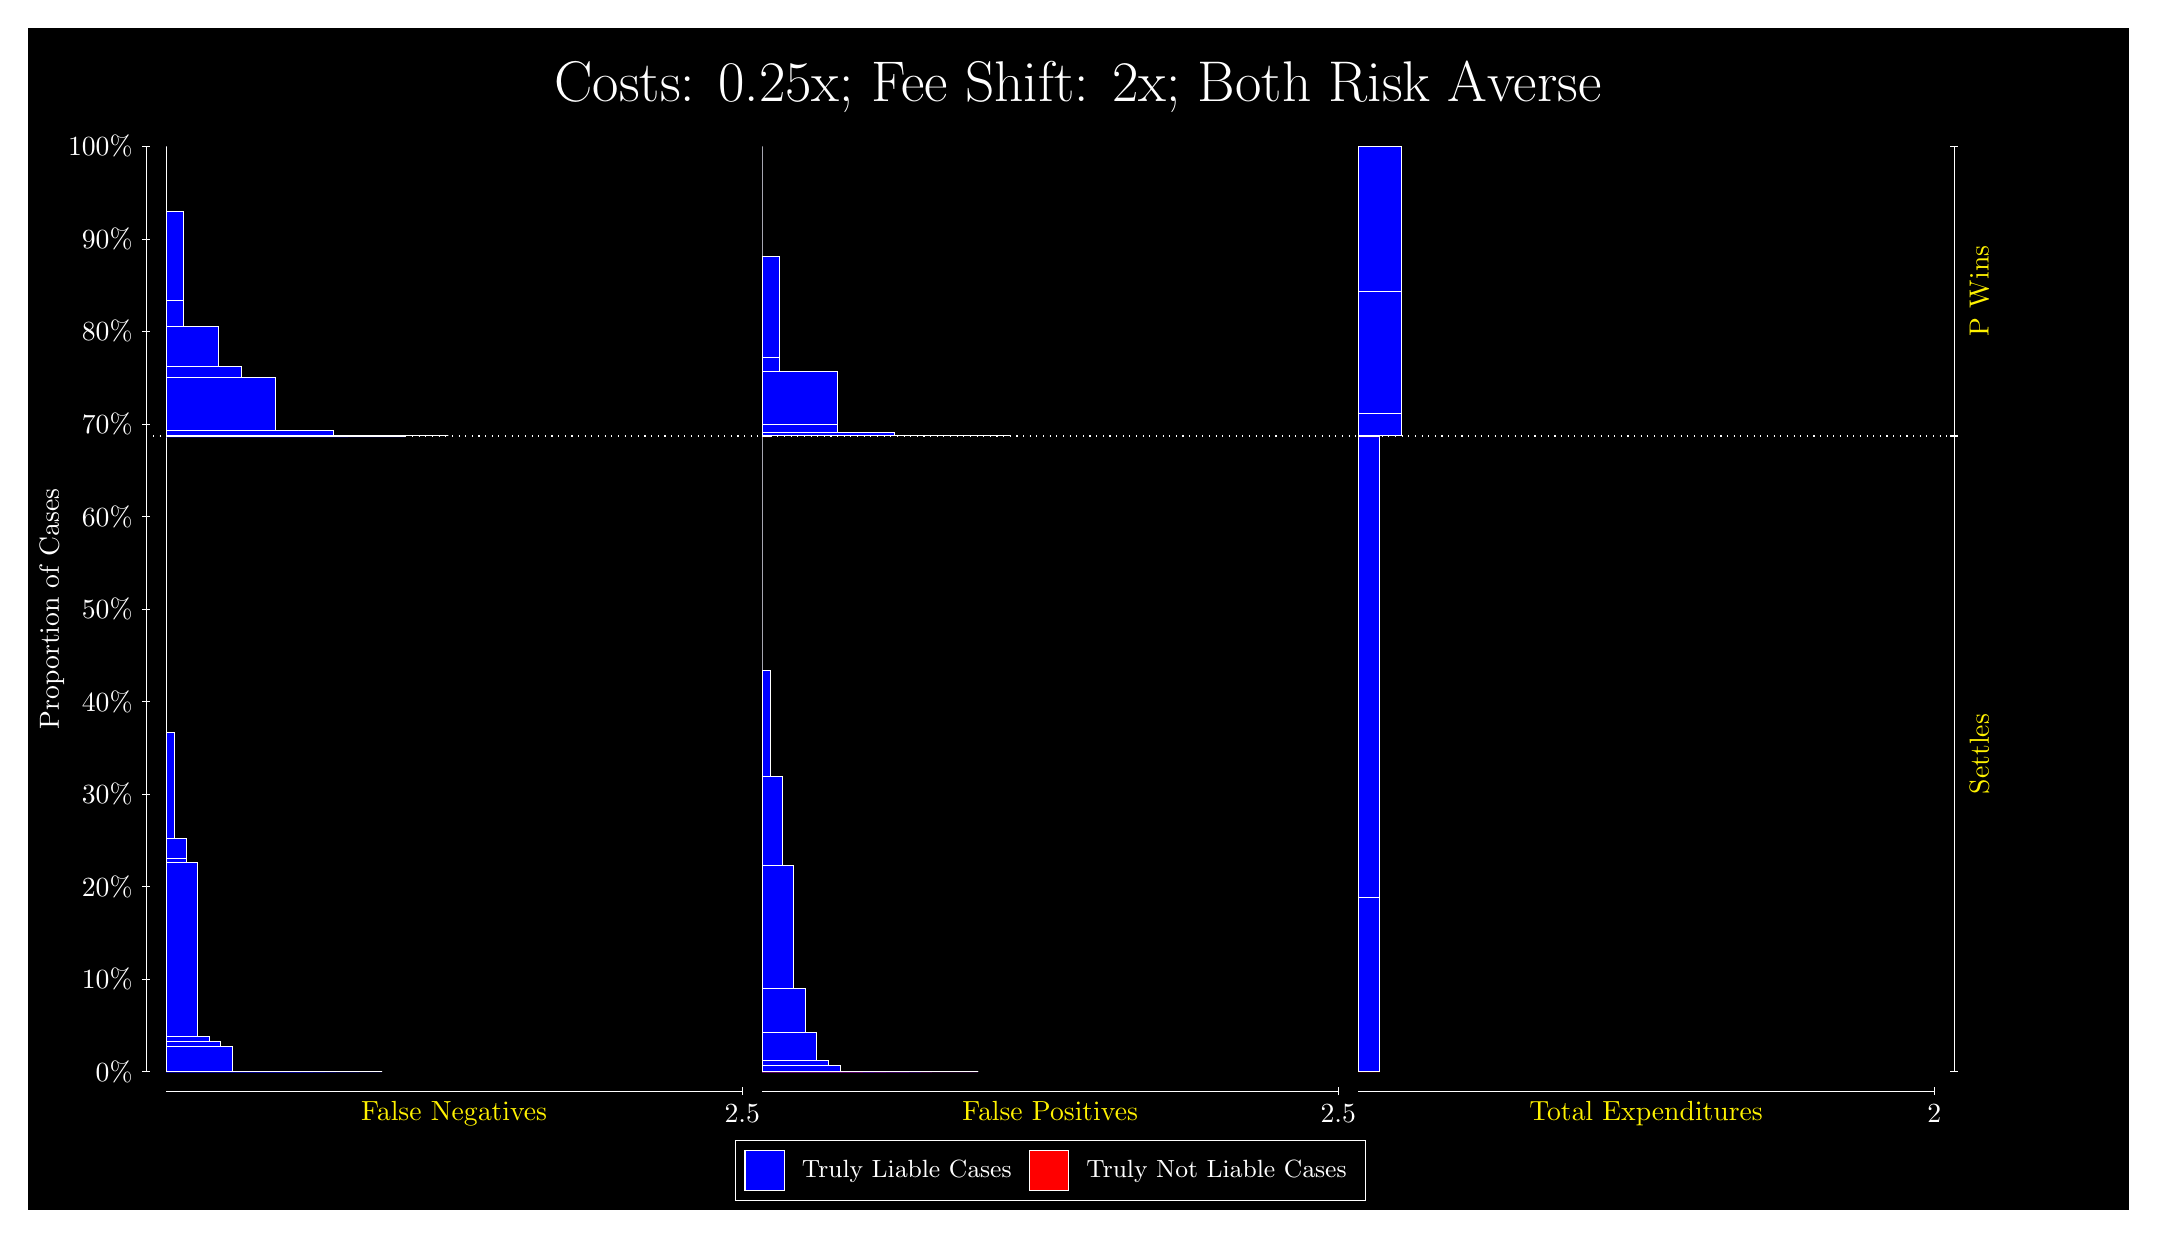
\begin{tikzpicture}
\draw[fill=black] (0,0) rectangle (26.667,15);
\draw[text=white] (0,13.5) rectangle (26.667,15) node[midway] {\huge Costs: 0.25x; Fee Shift: 2x; Both Risk Averse};
\draw[white, very thin] (1.5,1.75) -- (1.5,13.5);
\node[rotate=90, text=white, anchor=center] at (0.3, 7.625) {Proportion of Cases};
\draw[white, very thin] (1.45,1.75) -- (1.55,1.75);
\node[text=white, anchor=east] at (1.45, 1.75) {0\%};
\draw[white, very thin] (1.45,2.925) -- (1.55,2.925);
\node[text=white, anchor=east] at (1.45, 2.925) {10\%};
\draw[white, very thin] (1.45,4.1) -- (1.55,4.1);
\node[text=white, anchor=east] at (1.45, 4.1) {20\%};
\draw[white, very thin] (1.45,5.275) -- (1.55,5.275);
\node[text=white, anchor=east] at (1.45, 5.275) {30\%};
\draw[white, very thin] (1.45,6.45) -- (1.55,6.45);
\node[text=white, anchor=east] at (1.45, 6.45) {40\%};
\draw[white, very thin] (1.45,7.625) -- (1.55,7.625);
\node[text=white, anchor=east] at (1.45, 7.625) {50\%};
\draw[white, very thin] (1.45,8.8) -- (1.55,8.8);
\node[text=white, anchor=east] at (1.45, 8.8) {60\%};
\draw[white, very thin] (1.45,9.975) -- (1.55,9.975);
\node[text=white, anchor=east] at (1.45, 9.975) {70\%};
\draw[white, very thin] (1.45,11.15) -- (1.55,11.15);
\node[text=white, anchor=east] at (1.45, 11.15) {80\%};
\draw[white, very thin] (1.45,12.325) -- (1.55,12.325);
\node[text=white, anchor=east] at (1.45, 12.325) {90\%};
\draw[white, very thin] (1.45,13.5) -- (1.55,13.5);
\node[text=white, anchor=east] at (1.45, 13.5) {100\%};

\draw[white, very thin] (24.457,1.75) -- (24.457,13.5);
\draw[white, very thin] (24.407,1.75) -- (24.507,1.75);
\node[anchor=west] at (24.407, 1.75) {};
\draw[white, very thin] (24.407,9.8138) -- (24.507,9.8138);
\node[anchor=west] at (24.407, 9.8138) {};
\draw[white, very thin] (24.407,9.8292) -- (24.507,9.8292);
\node[anchor=west] at (24.407, 9.8292) {};
\draw[white, very thin] (24.407,13.5) -- (24.507,13.5);
\node[anchor=west] at (24.407, 13.5) {};

\draw[white, very thin, fill=blue] (1.75,1.75) rectangle (4.4946,1.75);
\draw[white, very thin, fill=blue] (1.75,1.75) rectangle (4.2018,1.75);
\draw[white, very thin, fill=blue] (1.75,1.75) rectangle (3.9091,1.75);
\draw[white, very thin, fill=blue] (1.75,1.75) rectangle (3.7627,1.75);
\draw[white, very thin, fill=blue] (1.75,1.75) rectangle (3.6163,1.75);
\draw[white, very thin, fill=blue] (1.75,1.75) rectangle (3.4699,1.75);
\draw[white, very thin, fill=blue] (1.75,1.75) rectangle (3.3236,1.7507);
\draw[white, very thin, fill=blue] (1.75,1.7507) rectangle (3.1772,1.7507);
\draw[white, very thin, fill=blue] (1.75,1.7507) rectangle (3.0308,1.7507);
\draw[white, very thin, fill=blue] (1.75,1.7507) rectangle (2.8844,1.7534);
\draw[white, very thin, fill=blue] (1.75,1.7534) rectangle (2.738,1.757);
\draw[white, very thin, fill=blue] (1.75,1.757) rectangle (2.5917,2.0683);
\draw[white, very thin, fill=blue] (1.75,2.0683) rectangle (2.4453,2.1281);
\draw[white, very thin, fill=blue] (1.75,2.1281) rectangle (2.2989,2.1915);
\draw[white, very thin, fill=blue] (1.75,2.1915) rectangle (2.1525,4.4058);
\draw[white, very thin, fill=blue] (1.75,4.4058) rectangle (2.0062,4.4641);
\draw[white, very thin, fill=blue] (1.75,4.4641) rectangle (2.0062,4.7125);
\draw[white, very thin, fill=blue] (1.75,4.7125) rectangle (1.8598,6.0602);
\draw[white, very thin, fill=red] (1.75,6.0602) rectangle (1.75,6.0602);
\draw[white, very thin, fill=blue] (1.75,6.0602) rectangle (1.75,9.8138);
\draw[white, very thin, fill=blue] (1.75,9.8138) rectangle (4.7873,9.8138);
\draw[white, very thin, fill=blue] (1.75,9.8138) rectangle (4.0554,9.8138);
\draw[white, very thin, fill=blue] (1.75,9.8138) rectangle (3.3236,9.8139);
\draw[white, very thin, fill=blue] (1.75,9.8139) rectangle (2.5917,9.8205);
\draw[white, very thin, fill=blue] (1.75,9.8205) rectangle (1.8598,9.8292);
\draw[white, very thin, fill=red] (1.75,9.8292) rectangle (1.75,9.8292);
\draw[white, very thin, fill=blue] (1.75,9.8292) rectangle (5.3362,9.8292);
\draw[white, very thin, fill=blue] (1.75,9.8292) rectangle (4.6044,9.8301);
\draw[white, very thin, fill=blue] (1.75,9.8301) rectangle (4.1652,9.8301);
\draw[white, very thin, fill=blue] (1.75,9.8301) rectangle (3.8725,9.8954);
\draw[white, very thin, fill=blue] (1.75,9.8954) rectangle (3.4333,9.8954);
\draw[white, very thin, fill=blue] (1.75,9.8954) rectangle (3.1406,10.565);
\draw[white, very thin, fill=blue] (1.75,10.565) rectangle (2.7015,10.568);
\draw[white, very thin, fill=blue] (1.75,10.568) rectangle (2.7015,10.704);
\draw[white, very thin, fill=blue] (1.75,10.704) rectangle (2.4087,11.22);
\draw[white, very thin, fill=blue] (1.75,11.22) rectangle (1.9696,11.544);
\draw[white, very thin, fill=blue] (1.75,11.544) rectangle (1.9696,12.68);
\draw[white, very thin, fill=red] (1.75,12.68) rectangle (1.75,12.68);
\draw[white, very thin, fill=blue] (1.75,12.68) rectangle (1.75,13.5);
\draw[white, very thin, fill=red] (9.3189,1.75) rectangle (12.063,1.75);
\draw[white, very thin, fill=blue] (9.3189,1.75) rectangle (12.063,1.75);
\draw[white, very thin, fill=red] (9.3189,1.75) rectangle (11.478,1.75);
\draw[white, very thin, fill=blue] (9.3189,1.75) rectangle (11.478,1.75);
\draw[white, very thin, fill=blue] (9.3189,1.75) rectangle (11.332,1.75);
\draw[white, very thin, fill=red] (9.3189,1.75) rectangle (11.185,1.75);
\draw[white, very thin, fill=blue] (9.3189,1.75) rectangle (11.185,1.75);
\draw[white, very thin, fill=red] (9.3189,1.75) rectangle (10.892,1.75);
\draw[white, very thin, fill=blue] (9.3189,1.75) rectangle (10.892,1.75);
\draw[white, very thin, fill=blue] (9.3189,1.75) rectangle (10.746,1.75);
\draw[white, very thin, fill=red] (9.3189,1.75) rectangle (10.6,1.75);
\draw[white, very thin, fill=blue] (9.3189,1.75) rectangle (10.6,1.7512);
\draw[white, very thin, fill=blue] (9.3189,1.7512) rectangle (10.453,1.7512);
\draw[white, very thin, fill=red] (9.3189,1.7512) rectangle (10.307,1.7512);
\draw[white, very thin, fill=blue] (9.3189,1.7512) rectangle (10.307,1.8349);
\draw[white, very thin, fill=blue] (9.3189,1.8349) rectangle (10.161,1.8937);
\draw[white, very thin, fill=red] (9.3189,1.8937) rectangle (10.014,1.8937);
\draw[white, very thin, fill=blue] (9.3189,1.8937) rectangle (10.014,2.2437);
\draw[white, very thin, fill=blue] (9.3189,2.2437) rectangle (10.014,2.2459);
\draw[white, very thin, fill=blue] (9.3189,2.2459) rectangle (9.8678,2.8125);
\draw[white, very thin, fill=red] (9.3189,2.8125) rectangle (9.7214,2.8125);
\draw[white, very thin, fill=blue] (9.3189,2.8125) rectangle (9.7214,4.3663);
\draw[white, very thin, fill=blue] (9.3189,4.3663) rectangle (9.7214,4.3668);
\draw[white, very thin, fill=blue] (9.3189,4.3668) rectangle (9.575,5.5037);
\draw[white, very thin, fill=blue] (9.3189,5.5037) rectangle (9.4287,6.8513);
\draw[white, very thin, fill=blue] (9.3189,6.8513) rectangle (9.3189,9.8138);
\draw[white, very thin, fill=red] (9.3189,9.8138) rectangle (9.4287,9.8138);
\draw[white, very thin, fill=blue] (9.3189,9.8138) rectangle (9.4287,9.8225);
\draw[white, very thin, fill=blue] (9.3189,9.8225) rectangle (9.3189,9.8292);
\draw[white, very thin, fill=red] (9.3189,9.8292) rectangle (12.466,9.8292);
\draw[white, very thin, fill=blue] (9.3189,9.8292) rectangle (12.466,9.8292);
\draw[white, very thin, fill=red] (9.3189,9.8292) rectangle (11.734,9.8292);
\draw[white, very thin, fill=blue] (9.3189,9.8292) rectangle (11.734,9.8296);
\draw[white, very thin, fill=red] (9.3189,9.8296) rectangle (11.002,9.8296);
\draw[white, very thin, fill=blue] (9.3189,9.8296) rectangle (11.002,9.8675);
\draw[white, very thin, fill=red] (9.3189,9.8675) rectangle (10.563,9.8675);
\draw[white, very thin, fill=blue] (9.3189,9.8675) rectangle (10.563,9.8675);
\draw[white, very thin, fill=red] (9.3189,9.8675) rectangle (10.27,9.8675);
\draw[white, very thin, fill=blue] (9.3189,9.8675) rectangle (10.27,9.9758);
\draw[white, very thin, fill=blue] (9.3189,9.9758) rectangle (10.27,10.648);
\draw[white, very thin, fill=red] (9.3189,10.648) rectangle (9.8312,10.648);
\draw[white, very thin, fill=blue] (9.3189,10.648) rectangle (9.8312,10.649);
\draw[white, very thin, fill=blue] (9.3189,10.649) rectangle (9.5384,10.816);
\draw[white, very thin, fill=blue] (9.3189,10.816) rectangle (9.5384,12.109);
\draw[white, very thin, fill=red] (9.3189,12.109) rectangle (9.3189,12.109);
\draw[white, very thin, fill=blue] (9.3189,12.109) rectangle (9.3189,13.5);
\draw[white, very thin, fill=red] (16.888,1.75) rectangle (17.162,1.75);
\draw[white, very thin, fill=blue] (16.888,1.75) rectangle (17.162,3.9657);
\draw[white, very thin, fill=red] (16.888,3.9657) rectangle (17.162,3.9657);
\draw[white, very thin, fill=blue] (16.888,3.9657) rectangle (17.162,9.8138);
\draw[white, very thin, fill=red] (16.888,9.8138) rectangle (17.162,9.8138);
\draw[white, very thin, fill=blue] (16.888,9.8138) rectangle (17.162,9.8292);
\draw[white, very thin, fill=red] (16.888,9.8292) rectangle (17.437,9.8292);
\draw[white, very thin, fill=blue] (16.888,9.8292) rectangle (17.437,10.107);
\draw[white, very thin, fill=red] (16.888,10.107) rectangle (17.437,10.107);
\draw[white, very thin, fill=blue] (16.888,10.107) rectangle (17.437,11.663);
\draw[white, very thin, fill=red] (16.888,11.663) rectangle (17.437,11.663);
\draw[white, very thin, fill=blue] (16.888,11.663) rectangle (17.437,13.5);
\draw[white, dotted] (1.5,9.8138) -- (24.457,9.8138);
\draw[white, dotted] (1.5,9.8292) -- (24.457,9.8292);
\draw[white, very thin] (1.75,1.5) -- (9.0689,1.5);
\node[text=yellow, anchor=north] at (5.4094, 1.5) {False Negatives};
\draw[white, very thin] (9.0689,1.45) -- (9.0689,1.55);
\node[text=white, anchor=north] at (9.0689, 1.45) {2.5};

\draw[white, very thin] (9.3189,1.5) -- (16.638,1.5);
\node[text=yellow, anchor=north] at (12.978, 1.5) {False Positives};
\draw[white, very thin] (16.638,1.45) -- (16.638,1.55);
\node[text=white, anchor=north] at (16.638, 1.45) {2.5};

\draw[white, very thin] (16.888,1.5) -- (24.207,1.5);
\node[text=yellow, anchor=north] at (20.547, 1.5) {Total Expenditures};
\draw[white, very thin] (24.207,1.45) -- (24.207,1.55);
\node[text=white, anchor=north] at (24.207, 1.45) {2};

\node[text=yellow, centered, rotate=90] at (24.777, 5.7819) {Settles};

\node[text=yellow, centered, rotate=90] at (24.777, 11.665) {P Wins};

\draw (12.978300999999998,1.5) node[draw=none] (baseCoordinate) {};
\begin{scope}[align=center]
        \matrix[scale=0.5, draw=white, below=0.5cm of baseCoordinate, nodes={draw}, column sep=0.1cm]{
            \node[rectangle, draw, minimum width=0.5cm, minimum height=0.5cm, fill=blue] {}; &
            \node[draw=none, font=\small, text=white] (B) {Truly Liable Cases}; &
            \node[rectangle, draw, minimum width=0.5cm, minimum height=0.5cm, fill=red] {}; &
            \node[draw=none, font=\small, text=white] (B) {Truly Not Liable Cases}; \\
            };
\end{scope}

\end{tikzpicture}
\end{document}